%Este trabalho está licenciado sob a Licença Creative Commons Atribuição-CompartilhaIgual 3.0 Não Adaptada. Para ver uma cópia desta licença, visite http://creativecommons.org/licenses/by-sa/3.0/ ou envie uma carta para Creative Commons, PO Box 1866, Mountain View, CA 94042, USA.

\documentclass[../livro.tex]{subfiles}  %%DM%%Escolher document class and options article, etc

%define o diretório principal
\providecommand{\dir}{..}

%%%%%%%%%%%%%%%%%%%%%%%%%%%%%%%%%%%%%%%%%%%%%
%%%%%%%%%%%%INICIO DO DOCUMENTO%%%%%%%%%%%%%%
%%%%%%%%%%%%%%%%%%%%%%%%%%%%%%%%%%%%%%%%%%%%%

\begin{document}

\chapter{Semana 10}


\section{Autovalores, autovetores e autoespaços associados}

Associados com uma transformação linear $T$ estão os seus autovetores, que, como veremos, são direções especiais para esta transformação $T$. Por esta razão, são também conhecidos como vetores próprios ou vetores característicos de $T$. Aparecem em muitas aplicações, pois nos ajudam a entender mais profundamente a transformação linear $T$.

Dada uma matriz \textit{quadrada} $A$ de ordem $n \times n$, com entradas reais, nós dizemos que um número $\lambda \in \mathbb{R}$ é um \textbf{autovalor} de $A$ quando existe um vetor \textit{não nulo} $\vec{v}$ tal que
\begin{equation}
A \vec{v} = \lambda \vec{v}.
\end{equation} Neste caso, $\vec{v}$ é dito um \textbf{autovetor} de $A$ associado a $\lambda$.

Geometricamente, $\vec{v}$ é um vetor que não muda de direção quando aplicamos a matriz $A$. No entanto, quando permitimos que $\lambda$ seja um número complexo, esta interpretação geométrica é perdida.

		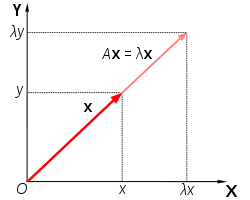
\includegraphics[width=1 \linewidth]{\dir/Semana10/semana10-eigen}

\noindent Ver também animação em \href{https://en.wikipedia.org/wiki/Eigenvalues_and_eigenvectors#Matrix_examples}{wikipedia.org}

\begin{example}
	Considere a matriz
	\begin{equation}
	A={\begin{bmatrix}2&0&0\\0&3&4\\0&4&9\end{bmatrix}}.
	\end{equation} Temos que $\lambda_1 = 2$ é um autovalor desta matriz, porque o vetor
	\begin{equation}
	\vec{v}_1 =
	{\begin{bmatrix}1\\0\\0\end{bmatrix}} \quad \text{ satisfaz } \quad {\begin{bmatrix}2&0&0\\0&3&4\\0&4&9\end{bmatrix}} {\begin{bmatrix}1\\0\\0\end{bmatrix}} = 2 \cdot {\begin{bmatrix}1\\0\\0\end{bmatrix}}.
	\end{equation} Assim, podemos dizer que $\vec{v}_1$ é um autovetor de $A$ associado ao autovalor $2$. Colocando de outra maneira, podemos dizer também que
	\begin{equation}
	\vec{v}_2 =
	{\begin{bmatrix}0\\1\\2\end{bmatrix}} \quad \text{ é um autovetor de $A$, pois } \quad {\begin{bmatrix}2&0&0\\0&3&4\\0&4&9\end{bmatrix}} {\begin{bmatrix}0\\1\\2\end{bmatrix}} = {\begin{bmatrix}0\\11\\22\end{bmatrix}} = 11 \cdot {\begin{bmatrix}0\\1\\2\end{bmatrix}}.
	\end{equation} Neste caso, concluimos também que $11$ é um autovalor de $A. \ \lhd$
\end{example}

Observamos que, se $\vec{v}$ for um autovetor de uma matriz $A$ associado a um autovalor $\lambda$, então qualquer múltiplo escalar $\alpha \vec{v}$ também é um autovetor de $A$ associado a $\lambda$:
\begin{equation}
A (\alpha \vec{v}) = \alpha A \vec{v} = \alpha \lambda \vec{v} = \lambda (\alpha \vec{v}).
\end{equation} Da mesma maneira, se dois vetores $\vec{v}$ e $\vec{w}$ forem autovetores associados a um mesmo autovalor $\lambda$, então a soma $\vec{v} + \vec{w}$ também é um autovetor associado a $\lambda$:
\begin{equation}
A (\vec{v} + \vec{w}) = A \vec{v} + A \vec{w} =  \lambda \vec{v} + \lambda \vec{w} = \lambda (\vec{v} + \vec{v}).
\end{equation} Logo, concluimos que o conjunto de todos os autovetores associados a um autovalor $\lambda$, união com o vetor nulo, forma um subespaço vetorial de $\mathbb{R}^n$, denominado \textbf{autoespaço} associado ao autovalor $\lambda$:
\begin{equation}
\text{autoespaço associado a } \lambda = \big\{ \vec{v} \in \mathbb{R}^n \, | \, \vec{v} \text{ é autovetor associado a } \lambda \big\} \cup \{\, \vec{0}\, \}.
\end{equation}

Vamos analisar uma forma de encontrar os autovalores de uma matriz $A$ de forma sistemática. Temos as seguintes equivalências:
\begin{align*}
& \lambda \text{ é um autovalor de $A$} \\
\iff & \text{existe } \vec{v} \neq \vec{0} \text{ tal que } A \vec{v} = \lambda \vec{v} \\
\iff & \text{existe } \vec{v} \neq \vec{0} \text{ tal que } (A - \lambda I)\vec{v} = \vec{0} \\
\iff & \text{o sistema homogêneo } (A - \lambda I)\vec{v} = \vec{0} \text{ admite solução não trivial} \\
\iff & A - \lambda I \text{ não é invertível} \\
\iff & \det (A - \lambda I) = 0.
\end{align*}
Esta última equação pode ser utilizada para encontrar os autovalores: são as raízes do \textbf{polinômio característico}
\begin{equation}
p(\lambda) = \det (A - \lambda I).
\end{equation} A equação $\det (A - \lambda I) = 0$ é também chamada de \textbf{equação característica}. Observe, pelas propriedades dos determinantes, que $p$ é de fato um polinômio e tem grau $n$, que é igual a ordem da matriz $A$. É assim consequência do Teorema Fundamental da Álgebra que existem no máximo $n$ autovalores reais (já que um polinômio de grau $n\ge 1$ possui exatamente $n$ raízes complexas).


\begin{example}\label{2x2}
	Vamos encontrar os autovalores de
	\begin{equation}
	A =
	\left[
	\begin{array}{cc}
	4 & 3 \\
	1 & 2 \\
	\end{array}
	\right].
	\end{equation} Precisamos calcular
	\begin{equation}
	\det\left[
	\begin{array}{cc}
	4-\lambda & 3 \\
	1 & 2-\lambda \\
	\end{array}
	\right] = (4-\lambda)(2-\lambda) - 3 \cdot 1 = \lambda^2 -6\lambda + 5,
	\end{equation} que tem raízes
	\begin{equation}
	\lambda = \frac{6 \pm \sqrt{36 - 20}}{2} = 3 \pm 2.
	\end{equation} Portanto, $A$ tem dois autovalores reais: $\lambda_1 = 1$ e $\lambda_2 = 5$.
\end{example}


\begin{example}\label{3x3}
	Encontrar os autovalores de
	\begin{equation}
	A =
	\left[
	\begin{array}{ccc}
	5 & 8 & 16 \\
	4 & 1 & 8 \\
	-4 & -4 & -11 \\
	\end{array}
	\right].
	\end{equation} Precisamos calcular
        \begin{align*}
	p(\lambda) = \det (A-\lambda I) & = \det
	\left[
	\begin{array}{ccc}
	5-\lambda & 8 & 16 \\
	4 & 1-\lambda & 8 \\
	-4 & -4 & -11-\lambda \\
	\end{array}
	\right] \\
	& = (5-\lambda) \cdot
	\left|
	\begin{array}{cc}
	1-\lambda & 8 \\
	-4 & -11-\lambda \\
	\end{array}
	\right| -8 \cdot
	\left|
	\begin{array}{cc}
	4 & 8 \\
	-4 & -11-\lambda \\
	\end{array}
	\right| + 16 \cdot
	\left|
	\begin{array}{cc}
	4 & 1-\lambda \\
	-4 & -4 \\
	\end{array}
	\right| \\
	& = (5-\lambda)\big[ (1-\lambda)(-11-\lambda) +32 \big] - 8 \big[ -44-4\lambda +32 \big] + 16 (-16 + 4 -4\lambda) \\
	& = (5-\lambda)\big[ \lambda^2 + 10 \lambda + 21 \big] + 32 \lambda + 12 \cdot 8 - 64\lambda - 12\cdot 16 \\
	& = -\lambda^3 - 5 \lambda^2 + 29 \lambda + 105  - 32 \lambda - 96 \\
	& = -\lambda^3 - 5 \lambda^2 - 3 \lambda + 9.
          \end{align*}
          As possíveis raízes racionais desse polinômio só podem ser os divisores do termo independente acima: $\pm 1, \pm 3, \pm9$. Verificamos que $1$ é raiz. Logo, dividindo $p(\lambda)$ por $\lambda - 1$:
	\begin{equation}
	-\lambda^3 - 5 \lambda^2 - 3 \lambda + 9 = -(\lambda - 1)(\lambda^2 + 6\lambda + 9) = -(\lambda - 1)(\lambda + 3)^2.
	\end{equation} Portanto, os autovalores de $A$ são $\lambda_1 = 1$ e $\lambda_2 = 3$. Observamos que $3$ é uma raiz de multiplicidade $2$ do polinômio característico. $\, \lhd$
\end{example}

Um grande problema é que, em geral, encontrar raízes de polinômios é difícil. De fato, mesmo quando o grau do polinômio é baixo, encontrar raízes de polinômios pode ser bastante complicado. Já há muito tempo é conhecido\footnote{Este resultado é uma consequência da famosa \href{https://pt.wikipedia.org/wiki/Teoria_de_Galois}{Teoria de Galois}.} que polinômios de grau $5$ ou mais podem não possuir fórmulas para cálculo de raízes a partir de radicais.

Por outro lado, uma vez que os autovalores são conhecidos, encontrar os autovetores é um cálculo direto: basta resolver o sistema linear homogêneo
\begin{equation}
\big( A - \lambda I \big) \vec{v} = \vec{0}.
\end{equation} Isto é o mesmo que dizer que o autoespaço associado a $\lambda$ é o espaço nulo $\operatorname{Nul} (A - \lambda I)$. Vejamos como encontrar os autoespaços das matrizes dos exemplos anteriores.

\begin{example}[de volta ao Exemplo \ref{2x2}]
	Para encontrar os autovetores de
	\begin{equation}
	A =
	\left[
	\begin{array}{cc}
	4 & 3 \\
	1 & 2 \\
	\end{array}
	\right]
	\end{equation} associados com o autovalor $\lambda_1 = 1$, vamos resolver o sistema homogêneo:
	\begin{equation}
	\left[
	\begin{array}{cc}
	4-\lambda & 3 \\
	1 & 2-\lambda \\
	\end{array}
	\right] \left[
	\begin{array}{c}
	v_1 \\
	v_2 \\
	\end{array}
	\right] = \left[
	\begin{array}{c}
	0 \\
	0 \\
	\end{array}
	\right] \leftrightsquigarrow
	\left[
	\begin{array}{cc}
	3 & 3 \\
	1 & 1 \\
	\end{array}
	\right] \left[
	\begin{array}{c}
	v_1 \\
	v_2 \\
	\end{array}
	\right] = \left[
	\begin{array}{c}
	0 \\
	0 \\
	\end{array}
	\right].
	\end{equation} Já que o sistema é homogêneo, não é necessário escrever a última coluna de zeros na matriz aumentada associada (no entanto, é necessário lembrar que há uma coluna de zeros). Por escalonamento
	\begin{equation}
	\left[
	\begin{array}{cc}
	3 & 3 \\
	1 & 1 \\
	\end{array}
	\right] \sim
	\left[
	\begin{array}{cc}
	1 & 1 \\
	0 & 0 \\
	\end{array}
	\right] \leftrightsquigarrow
	\left\{
	\begin{array}{ll}
	v_1 + v_2 = 0 \\
	\hbox{1 variável livre.}
	\end{array}
	\right.
	\end{equation} Em forma vetorial paramétrica:
	\begin{equation}
	\left[
	\begin{array}{c}
	v_1 \\
	v_2 \\
	\end{array}
	\right] =
	\left[
	\begin{array}{c}
	-v_2 \\
	v_2 \\
	\end{array}
	\right] = v_2
	\left[
	\begin{array}{c}
	-1 \\
	1 \\
	\end{array}
	\right] \implies \operatorname{Nul} (A - I) = \Span \left\{ \left[
	\begin{array}{c}
	-1 \\
	1 \\
	\end{array}
	\right] \right\}.
	\end{equation}
	
	Para encontrar os autovetores associados a $\lambda_2 = 5$, resolvemos
	\begin{equation}
	\left[
	\begin{array}{cc}
	4-\lambda & 3 \\
	1 & 2-\lambda \\
	\end{array}
	\right] =
	\left[
	\begin{array}{cc}
	-1 & 3 \\
	1 & -3 \\
	\end{array}
	\right] \sim
	\left[
	\begin{array}{cc}
	1 & -3 \\
	0 &  0 \\
	\end{array}
	\right] \leftrightsquigarrow
	\left\{
	\begin{array}{ll}
	v_1 - 3 v_2 = 0 \\
	\hbox{1 variável livre.}
	\end{array}
	\right.
	\end{equation} Em forma vetorial paramétrica:
	\begin{equation}
	\left[
	\begin{array}{c}
	v_1 \\
	v_2 \\
	\end{array}
	\right] =
	\left[
	\begin{array}{c}
	3v_2 \\
	v_2 \\
	\end{array}
	\right] = v_2
	\left[
	\begin{array}{c}
	3 \\
	1 \\
	\end{array}
	\right] \implies \operatorname{Nul} (A - 5 I) = \Span \left\{ \left[
	\begin{array}{c}
	3 \\
	1 \\
	\end{array}
	\right] \right\}.
	\end{equation}
\end{example}

\begin{example}[de volta ao Exemplo \ref{3x3}]
	Vamos encontrar os autovetores de
	\begin{equation}
	A =
	\left[
	\begin{array}{ccc}
	5 & 8 & 16 \\
	4 & 1 & 8 \\
	-4 & -4 & -11 \\
	\end{array}
	\right].
	\end{equation}
	
	\begin{itemize}
		\item associados com o autovalor $\lambda_1 = 1$, vamos resolver o sistema homogêneo:
		\begin{equation}
		\left[
		\begin{array}{ccc}
		5-\lambda_1 & 8 & 16 \\
		4 & 1-\lambda_1 & 8 \\
		-4 & -4 & -11-\lambda_1 \\
		\end{array}
		\right] \left[
		\begin{array}{ccc}
		v_1 \\
		v_2 \\
		v_3 \\
		\end{array}
		\right] = \left[
		\begin{array}{ccc}
		0 \\
		0 \\
		0 \\
		\end{array}
		\right].
		\end{equation} Por escalonamento,
		\begin{equation}
		\left[
		\begin{array}{ccc}
		4 &  8 & 16 \\
		4 &  0 & 8 \\
		-4 & -4 & -12 \\
		\end{array}
		\right] \sim \left[
		\begin{array}{ccc}
		1 &  2 & 4 \\
		0 & -8 & -8 \\
		0 &  4 & 4 \\
		\end{array}
		\right] \sim \left[
		\begin{array}{ccc}
		1 &  2 & 4 \\
		0 &  1 & 1 \\
		0 &  0 & 0 \\
		\end{array}
		\right] \sim \left[
		\begin{array}{ccc}
		1 &  0 & 2 \\
		0 &  1 & 1 \\
		0 &  0 & 0 \\
		\end{array}
		\right] \leftrightsquigarrow
		\left\{
		\begin{array}{ll}
		v_1 + 2 v_3 = 0 \\
		v_2 + v_3 = 0 \\
		v_3  \hbox{ livre}
		\end{array}
		\right.
		\end{equation} Em forma paramétrica, os autovetores são
		\begin{equation}
		\left[
		\begin{array}{ccc}
		v_1 \\
		v_2 \\
		v_3 \\
		\end{array}
		\right] =
		\left[
		\begin{array}{ccc}
		-2v_3 \\
		-v_3 \\
		v_3 \\
		\end{array}
		\right] = v_3
		\left[
		\begin{array}{ccc}
		-2 \\
		-1 \\
		1 \\
		\end{array}
		\right]  \implies \operatorname{Nul} (A - I) = \Span \left\{ \left[
		\begin{array}{c}
		-2 \\
		-1 \\
		1 \\
		\end{array}
		\right] \right\}.
		\end{equation}
		\item associados com o autovalor $\lambda_2 = -3$, vamos resolver o sistema homogêneo:
		\begin{equation}
		\left[
		\begin{array}{ccc}
		5-\lambda_2 & 8 & 16 \\
		4 & 1-\lambda_2 & 8 \\
		-4 & -4 & -11-\lambda_2 \\
		\end{array}
		\right] \left[
		\begin{array}{ccc}
		v_1 \\
		v_2 \\
		v_3 \\
		\end{array}
		\right] = \left[
		\begin{array}{ccc}
		0 \\
		0 \\
		0 \\
		\end{array}
		\right].
		\end{equation} Por escalonamento,
		\begin{equation}
		\left[
		\begin{array}{ccc}
		8 &  8 & 16 \\
		4 &  4 & 8 \\
		-4 & -4 & -8 \\
		\end{array}
		\right] \sim \left[
		\begin{array}{ccc}
		1 &  1 & 2 \\
		0 &  0 & 0 \\
		0 &  0 & 0 \\
		\end{array}
		\right] \leftrightsquigarrow
		\left\{
		\begin{array}{ll}
		v_1 + v_2 + 2v_3 = 0 \\
		\hbox{2 variáveis livres}
		\end{array}
		\right.
		\end{equation} Em forma paramétrica, os autovetores são
		\begin{equation}
		\left[
		\begin{array}{ccc}
		v_1 \\
		v_2 \\
		v_3 \\
		\end{array}
		\right] =
		\left[
		\begin{array}{ccc}
		- v_2 - 2 v_3 \\
		v_2 \\
		v_3 \\
		\end{array}
		\right] = v_2
		\left[
		\begin{array}{ccc}
		-1 \\
		1 \\
		0 \\
		\end{array}
		\right] + v_3
		\left[
		\begin{array}{ccc}
		-2 \\
		0 \\
		1 \\
		\end{array}
		\right] \implies \operatorname{Nul} (A - I) = \Span \left\{ \left[
		\begin{array}{c}
		-1 \\
		1 \\
		0 \\
		\end{array}
		\right], \left[
		\begin{array}{ccc}
		-2 \\
		0 \\
		1 \\
		\end{array}
		\right] \right\}. \lhd
		\end{equation}
	\end{itemize}
\end{example}

Observamos que, nos exemplos anteriores, a dimensão do autoespaço associado ficou igual à multiplicidade do autovalor. \textbf{Isto nem sempre é verdade}. Como exercício, verifique que a dimensão do autoespaço associado ao autovalor $\lambda = 1$ da matriz
\begin{equation}
\begin{bmatrix}
1 & 1 \\ 0 & 1
\end{bmatrix}
\end{equation} é igual a $1$, embora a multiplicidade do autovalor seja $2$.

De forma geral, chamamos a multiplicidade do autovalor de \textbf{multiplicidade algébrica}, enquanto que a dimensão do autoespaço associado é chamada de \textbf{multiplicidade geométrica}.

\subsection*{Exercícios resolvidos}

\construirExeresol

\subsection*{Exercícios}

\construirExer

\section{Diagonalização}

Matrizes diagonais são matrizes da forma
\begin{equation}
\begin{bmatrix}
\lambda_1 & 0 & 0 & \cdots & 0 \\
0 & \lambda_2 & 0 & \cdots & 0 \\
0 & 0 & \lambda_3 & \cdots & 0 \\
\vdots & \vdots & \vdots & \ddots & \vdots \\
0 & 0 & 0 & \cdots & \lambda_n \\
\end{bmatrix}.
\end{equation} Já que são triangulares, seus autovalores são os elementos da diagonal principal. Observamos também que os autovetores associados são os elementos da base canônica de $\mathbb{R}^n$.

Na realidade, o fato de se conseguir formar uma base com autovetores de uma matriz está intimamente relacionado com se obter uma matriz diagonal semelhante a $A$. De fato, vamos justificar que, sempre que for possível formar uma base do espaço $\mathbb{R}^n$ apenas com autovetores de uma matriz quadrada $A$, então é possível fazer uma mudança de base de modo que a obter uma matriz diagonal, com os autovalores na diagonal principal. Este procedimento é chamado de \textbf{diagonalização} da matriz $A$, por motivos óbvios. O método, que é surpreendentemente simples (mas, na prática, trabalhoso), consiste em montar uma matriz $P$ com os autovetores de $A$ e efetuar multiplicações de matrizes:
\begin{equation}
P = \begin{bmatrix}
| & | &  & | \\
\vec{v}_1 & \vec{v}_2 & \cdots & \vec{v}_n \\
| & | &  & |\\
\end{bmatrix} \implies P^{-1} A P = D = \begin{bmatrix}
\lambda_1 & 0  & \cdots & 0 \\
0 & \lambda_2  & \cdots & 0 \\
\vdots & \vdots & \ddots & \vdots \\
0 & 0 & \cdots & \lambda_n \\
\end{bmatrix}.
\end{equation}

\begin{proof}[Justificativa do método de diagonalização]
Vamos verificar que $P^{-1} A P = D$ mostrando que as colunas da matriz $P^{-1} A P$ são iguais as colunas de $D$. Pela forma que construimos a matriz $P$, sabemos que a primeira coluna de $P$ é $\vec{v}_1$: 
\begin{equation}
P \vec{e}_1 = \vec{v}_1 \qquad \qquad \text{ou, ainda, } \qquad  \vec{e}_1 = P^{-1} \vec{v}_1.
\end{equation} Assim, já que $A \vec{v}_1 = \lambda_1 \vec{v}_1$, temos
\begin{equation}
\begin{split}
\text{primeira coluna de } P^{-1} A P  & = P^{-1} A P \vec{e}_1 \\
                                       & = P^{-1} A \vec{v}_1 \\
                                       & = P^{-1} \lambda_1 \vec{v}_1 \\
                                       & = \lambda_1 P^{-1} \vec{v}_1 \\
                                       & = \lambda_1 \vec{e}_1 \\
                                       & = \text{primeira coluna de } D.
\end{split}
\end{equation}
Este mesmo raciocício, repetido $n$ vezes, para cada uma das colunas, prova que todas as colunas são iguais; portanto, $P^{-1} A P = D$.
\end{proof}

\begin{example}[de volta ao Exemplo \ref{3x3}]\label{exp:3x3denovo}
	Vimos que, para a matriz
	\begin{equation}
	A =
	\left[
	\begin{array}{ccc}
	5 & 8 & 16 \\
	4 & 1 & 8 \\
	-4 & -4 & -11 \\
	\end{array}
	\right],
	\end{equation} temos autovalores $\lambda_1 = 1$ e $\lambda_2 = -3$ e autoespaços associados:
	\begin{equation}
	\operatorname{Nul} (A - I) = \Span \left\{ \left[
	\begin{array}{c}
	-2 \\
	-1 \\
	1 \\
	\end{array}
	\right] \right\}; \qquad \operatorname{Nul} (A - I) = \Span \left\{ \left[
	\begin{array}{c}
	-1 \\
	1 \\
	0 \\
	\end{array}
	\right], \left[
	\begin{array}{ccc}
	-2 \\
	0 \\
	1 \\
	\end{array}
	\right] \right\}.
	\end{equation} Montamos a matriz
	\begin{equation}
	P =
	\begin{bmatrix}
	-2&-1&-2 \\ -1&1&0 \\ 1&0&1
	\end{bmatrix}
	\end{equation} Por escalonamento, podemos calcular a matriz inversa
	\begin{equation}
	P^{-1} =
	\begin{bmatrix}
	-1&-1&-2 \\ -1&0&-2 \\ 1&1&3
	\end{bmatrix}
	\end{equation} e temos
          \begin{align*}
	P^{-1} A P & =
	\begin{bmatrix}
	-1&-1&-2 \\ -1&0&-2 \\ 1&1&3
	\end{bmatrix}
	\begin{bmatrix}
	5 & 8 & 16 \\ 4 & 1 & 8 \\ -4 & -4 & -11 \\
	\end{bmatrix}
	\begin{bmatrix}
	-2&-1&-2 \\ -1&1&0 \\ 1&0&1
	\end{bmatrix} \\
	& =
	\begin{bmatrix}
	-1&-1&-2 \\ 3&0&6 \\ -3&-3&-9
	\end{bmatrix}
	\begin{bmatrix}
	-2&-1&-2 \\ -1&1&0 \\ 1&0&1
	\end{bmatrix} =
	\begin{bmatrix}
	1&0&0 \\ 0&-3&0 \\ 0&0&-3
	\end{bmatrix}. \ \lhd
          \end{align*}
\end{example}

Embora o método de diagonalização seja bastante transparente, pois basta seguir uma sequência de passos, ele é muito trabalhoso! Não devemos nos iludir com a aparente simplicidade das contas no Exemplo \ref{exp:3x3denovo}, pois as contas já haviam sido feitas anteriormente (além de que ``escondemos'' o cálculo da inversa $P^{-1}$). Na totalidade, os passos envolvem:
\begin{itemize}
\item Calcular o polinômio característico $p(\lambda) = \det (A - \lambda I)$. Aqui já entra uma quantidade significativa de cálculos, cuja quantidade aumenta de acordo com a dimensão do problema;
\item Encontrar as raízes do polinômio característico. Este passo pode ser muito complicado, já que muitas vezes não é possível encontrar raízes explicitamente;
\item Depois de conhecidos os autovalores, calcular cada um dos autoespaços associados, o que demanda a resolução de tantos sistemas lineares quantos forem os autovalores distintos da matriz;
\item Caso todos os geradores de todos os autoespaços formem uma base para o espaço $\mathbb{R}^n$, a matriz $A$ é diagonalizável e formamos a matriz $P$ como indicado acima;
\item Observe que, se estivermos apenas interessados em encontrar uma base de autovetores e uma matriz diagonal equivalente a $A$, então não há necessidade de se calcular $P^{-1}$, pois já sabemos que o método funciona e que $P^{-1} AP = D$. No entanto, uma descrição mais completa pode ser necessária nas principais aplicações, de modo que ainda seria preciso uma quantidade grande de cálculos para determinar a matriz $P^{-1}$.
\end{itemize}

Nem todas as matrizes são diagonalizáveis, como acima. Já vimos que isto é possível quando uma base de autovetores existe. No exemplo
\begin{equation}
A = \begin{bmatrix}
2&1 \\ 0&2
\end{bmatrix}
\end{equation} não há dois autovetores linearmente independentes e, portanto, não é possível diagonalizar a matriz $A$.


\vspace{0.3cm}

Em geral, valem as seguintes propriedades: seja $A$ uma matriz de orden $n \times n$. Então:
\begin{itemize}
	\item Se $A$ possui $n$ autovalores reais distintos, então $A$ possui uma base de autovetores e é diagonalizável, pois possui um autovetor associado a cada um dos seus autovalores distintos.
	\item No caso de $A$ possuir autovalores reais com multiplicidade maior do que $1$, $A$ apenas será diagonalizável se cada autovalor de multiplicidade $k$ tiver $k$ autovetores linearmente independentes. Em outras palavras, só será possível formar uma base de autovetores de $A$ quando 
	\begin{equation}
	\operatorname{dim} \operatorname{Nul} (A - \lambda I) = \text{ multiplicidade do autovalor } \lambda.
	\end{equation} Na notação introduzida não seção anterior, isto é o mesmo que dizer que, se $A$ for diagonalizável, então as multiplicidades algébrica e geométrica são iguais.
	\item Caso $\dim \operatorname{Nul} (A - \lambda I)$ seja menor do que a multiplicidade do autovalor $\lambda$ ou $A$ possua autovalores complexos, então $A$ não é diagonalizável.
\end{itemize}


\begin{example}
	A matriz
	\begin{equation}
	A = \begin{bmatrix}
	2&1 \\ -1&2
	\end{bmatrix}
	\end{equation} tem polinômio característico 
	\begin{equation}
	p(\lambda) = \det \begin{bmatrix}
	2-\lambda&1 \\ -1&2-\lambda
	\end{bmatrix} = (2-\lambda)^2 +1 = \lambda^2 -4\lambda +5
	\end{equation} cujas raízes são $\lambda_1 = \frac{4 + 3i}{2}$ e $\lambda_2 = \frac{4 - 3i}{2}$. Logo, $A$ não é diagonalizável.
\end{example}

\subsection*{Exercícios resolvidos}

\construirExeresol

\subsection*{Exercícios}

\construirExer

\section{Exercícios finais}

\construirExer

\end{document} 